% Created by tikzDevice version 0.6.2-92-0ad2792 on 2013-01-10 19:18:55
% !TEX encoding = UTF-8 Unicode
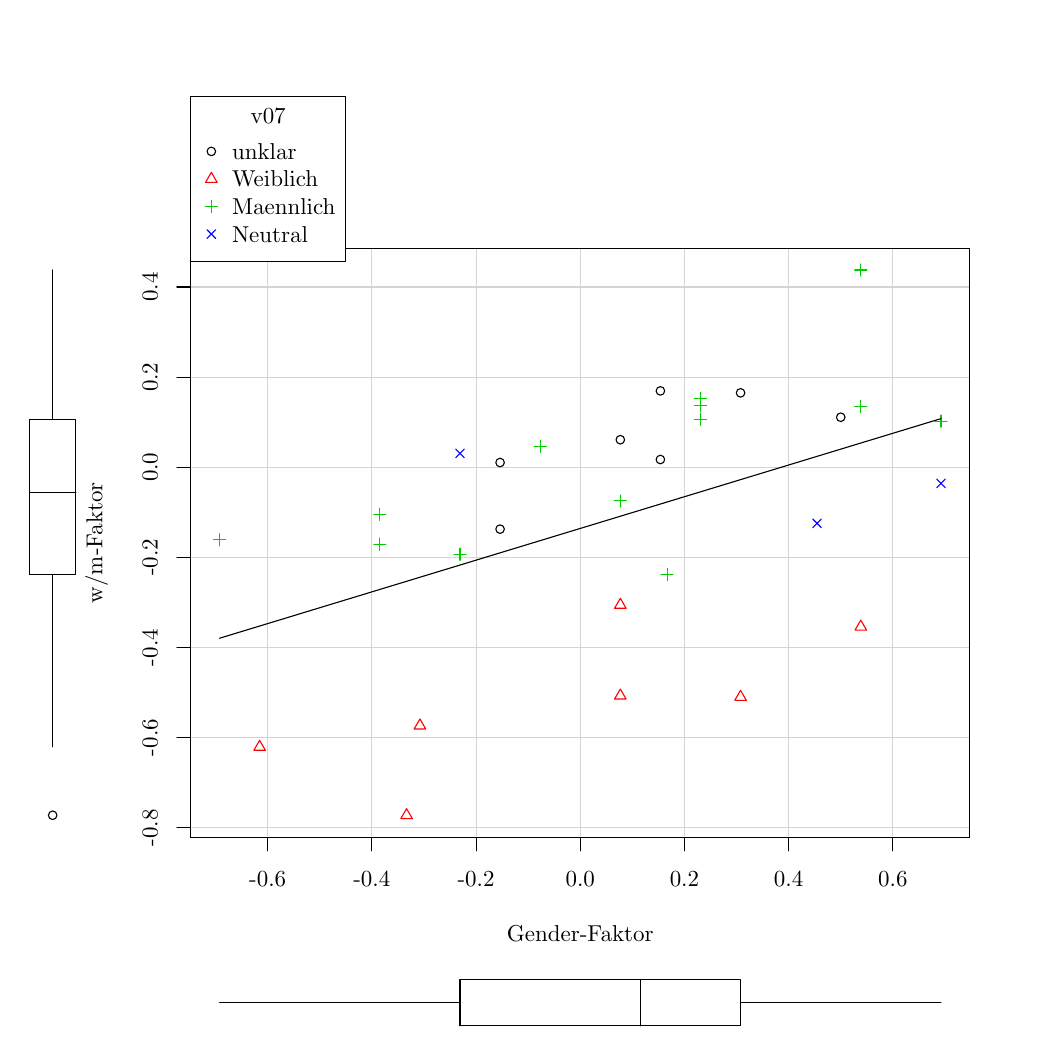
\begin{tikzpicture}[x=1pt,y=1pt]
\definecolor[named]{fillColor}{rgb}{1.00,1.00,1.00}
\path[use as bounding box,fill=fillColor,fill opacity=0.00] (0,0) rectangle (361.35,361.35);
\begin{scope}
\path[clip] (  0.00, 68.86) rectangle ( 18.07,281.67);
\definecolor[named]{drawColor}{rgb}{0.00,0.00,0.00}

\path[draw=drawColor,line width= 0.4pt,line join=round,line cap=round] (  0.67,163.73) --
	( 17.40,163.73) --
	( 17.40,219.81) --
	(  0.67,219.81) --
	(  0.67,163.73);

\path[draw=drawColor,line width= 0.4pt,line join=round,line cap=round] (  0.67,193.51) --
	( 17.40,193.51);

\path[draw=drawColor,line width= 0.4pt,line join=round,line cap=round] (  9.03,101.44) --
	(  9.03,163.73);

\path[draw=drawColor,line width= 0.4pt,line join=round,line cap=round] (  9.03,219.81) --
	(  9.03,273.79);

\path[draw=drawColor,line width= 0.4pt,line join=round,line cap=round] (  9.03, 76.75) circle (  1.55);
\end{scope}
\begin{scope}
\path[clip] ( 58.90,  0.00) rectangle (340.43, 18.07);
\definecolor[named]{drawColor}{rgb}{0.00,0.00,0.00}

\path[draw=drawColor,line width= 0.4pt,line join=round,line cap=round] (156.22,  0.67) --
	(156.22, 17.40) --
	(257.60, 17.40) --
	(257.60,  0.67) --
	(156.22,  0.67);

\path[draw=drawColor,line width= 0.4pt,line join=round,line cap=round] (221.39,  0.67) --
	(221.39, 17.40);

\path[draw=drawColor,line width= 0.4pt,line join=round,line cap=round] ( 69.33,  9.03) --
	(156.22,  9.03);

\path[draw=drawColor,line width= 0.4pt,line join=round,line cap=round] (257.60,  9.03) --
	(330.01,  9.03);
\end{scope}
\begin{scope}
\path[clip] (  0.00,  0.00) rectangle (361.35,361.35);
\definecolor[named]{drawColor}{rgb}{0.00,0.00,0.00}

\path[draw=drawColor,line width= 0.4pt,line join=round,line cap=round] ( 86.71, 68.86) -- (312.63, 68.86);

\path[draw=drawColor,line width= 0.4pt,line join=round,line cap=round] ( 86.71, 68.86) -- ( 86.71, 63.88);

\path[draw=drawColor,line width= 0.4pt,line join=round,line cap=round] (124.36, 68.86) -- (124.36, 63.88);

\path[draw=drawColor,line width= 0.4pt,line join=round,line cap=round] (162.02, 68.86) -- (162.02, 63.88);

\path[draw=drawColor,line width= 0.4pt,line join=round,line cap=round] (199.67, 68.86) -- (199.67, 63.88);

\path[draw=drawColor,line width= 0.4pt,line join=round,line cap=round] (237.32, 68.86) -- (237.32, 63.88);

\path[draw=drawColor,line width= 0.4pt,line join=round,line cap=round] (274.98, 68.86) -- (274.98, 63.88);

\path[draw=drawColor,line width= 0.4pt,line join=round,line cap=round] (312.63, 68.86) -- (312.63, 63.88);

\node[text=drawColor,anchor=base,inner sep=0pt, outer sep=0pt, scale=  0.83] at ( 86.71, 50.94) {-0.6};

\node[text=drawColor,anchor=base,inner sep=0pt, outer sep=0pt, scale=  0.83] at (124.36, 50.94) {-0.4};

\node[text=drawColor,anchor=base,inner sep=0pt, outer sep=0pt, scale=  0.83] at (162.02, 50.94) {-0.2};

\node[text=drawColor,anchor=base,inner sep=0pt, outer sep=0pt, scale=  0.83] at (199.67, 50.94) {0.0};

\node[text=drawColor,anchor=base,inner sep=0pt, outer sep=0pt, scale=  0.83] at (237.32, 50.94) {0.2};

\node[text=drawColor,anchor=base,inner sep=0pt, outer sep=0pt, scale=  0.83] at (274.98, 50.94) {0.4};

\node[text=drawColor,anchor=base,inner sep=0pt, outer sep=0pt, scale=  0.83] at (312.63, 50.94) {0.6};

\path[draw=drawColor,line width= 0.4pt,line join=round,line cap=round] ( 58.90, 72.24) -- ( 58.90,267.62);

\path[draw=drawColor,line width= 0.4pt,line join=round,line cap=round] ( 58.90, 72.24) -- ( 53.92, 72.24);

\path[draw=drawColor,line width= 0.4pt,line join=round,line cap=round] ( 58.90,104.81) -- ( 53.92,104.81);

\path[draw=drawColor,line width= 0.4pt,line join=round,line cap=round] ( 58.90,137.37) -- ( 53.92,137.37);

\path[draw=drawColor,line width= 0.4pt,line join=round,line cap=round] ( 58.90,169.93) -- ( 53.92,169.93);

\path[draw=drawColor,line width= 0.4pt,line join=round,line cap=round] ( 58.90,202.49) -- ( 53.92,202.49);

\path[draw=drawColor,line width= 0.4pt,line join=round,line cap=round] ( 58.90,235.05) -- ( 53.92,235.05);

\path[draw=drawColor,line width= 0.4pt,line join=round,line cap=round] ( 58.90,267.62) -- ( 53.92,267.62);

\node[text=drawColor,rotate= 90.00,anchor=base,inner sep=0pt, outer sep=0pt, scale=  0.83] at ( 46.95, 72.24) {-0.8};

\node[text=drawColor,rotate= 90.00,anchor=base,inner sep=0pt, outer sep=0pt, scale=  0.83] at ( 46.95,104.81) {-0.6};

\node[text=drawColor,rotate= 90.00,anchor=base,inner sep=0pt, outer sep=0pt, scale=  0.83] at ( 46.95,137.37) {-0.4};

\node[text=drawColor,rotate= 90.00,anchor=base,inner sep=0pt, outer sep=0pt, scale=  0.83] at ( 46.95,169.93) {-0.2};

\node[text=drawColor,rotate= 90.00,anchor=base,inner sep=0pt, outer sep=0pt, scale=  0.83] at ( 46.95,202.49) {0.0};

\node[text=drawColor,rotate= 90.00,anchor=base,inner sep=0pt, outer sep=0pt, scale=  0.83] at ( 46.95,235.05) {0.2};

\node[text=drawColor,rotate= 90.00,anchor=base,inner sep=0pt, outer sep=0pt, scale=  0.83] at ( 46.95,267.62) {0.4};

\path[draw=drawColor,line width= 0.4pt,line join=round,line cap=round] ( 58.90, 68.86) --
	(340.43, 68.86) --
	(340.43,281.67) --
	( 58.90,281.67) --
	( 58.90, 68.86);
\end{scope}
\begin{scope}
\path[clip] ( 18.07, 18.07) rectangle (361.35,361.35);
\definecolor[named]{drawColor}{rgb}{0.00,0.00,0.00}

\node[text=drawColor,anchor=base,inner sep=0pt, outer sep=0pt, scale=  0.83] at (199.67, 31.02) {Gender-Faktor};

\node[text=drawColor,rotate= 90.00,anchor=base,inner sep=0pt, outer sep=0pt, scale=  0.83] at ( 27.03,175.27) {w/m-Faktor};
\end{scope}
\begin{scope}
\path[clip] ( 58.90, 68.86) rectangle (340.43,281.67);
\definecolor[named]{drawColor}{rgb}{0.83,0.83,0.83}

\path[draw=drawColor,line width= 0.4pt,line join=round,line cap=round] ( 86.71, 68.86) -- ( 86.71,281.67);

\path[draw=drawColor,line width= 0.4pt,line join=round,line cap=round] (124.36, 68.86) -- (124.36,281.67);

\path[draw=drawColor,line width= 0.4pt,line join=round,line cap=round] (162.02, 68.86) -- (162.02,281.67);

\path[draw=drawColor,line width= 0.4pt,line join=round,line cap=round] (199.67, 68.86) -- (199.67,281.67);

\path[draw=drawColor,line width= 0.4pt,line join=round,line cap=round] (237.32, 68.86) -- (237.32,281.67);

\path[draw=drawColor,line width= 0.4pt,line join=round,line cap=round] (274.98, 68.86) -- (274.98,281.67);

\path[draw=drawColor,line width= 0.4pt,line join=round,line cap=round] (312.63, 68.86) -- (312.63,281.67);

\path[draw=drawColor,line width= 0.4pt,line join=round,line cap=round] ( 58.90, 72.24) -- (340.43, 72.24);

\path[draw=drawColor,line width= 0.4pt,line join=round,line cap=round] ( 58.90,104.81) -- (340.43,104.81);

\path[draw=drawColor,line width= 0.4pt,line join=round,line cap=round] ( 58.90,137.37) -- (340.43,137.37);

\path[draw=drawColor,line width= 0.4pt,line join=round,line cap=round] ( 58.90,169.93) -- (340.43,169.93);

\path[draw=drawColor,line width= 0.4pt,line join=round,line cap=round] ( 58.90,202.49) -- (340.43,202.49);

\path[draw=drawColor,line width= 0.4pt,line join=round,line cap=round] ( 58.90,235.05) -- (340.43,235.05);

\path[draw=drawColor,line width= 0.4pt,line join=round,line cap=round] ( 58.90,267.62) -- (340.43,267.62);
\end{scope}
\begin{scope}
\path[clip] (  0.00,  0.00) rectangle (361.35,361.35);
\definecolor[named]{drawColor}{rgb}{0.00,0.00,0.00}

\path[draw=drawColor,line width= 0.4pt,line join=round,line cap=round] ( 58.90, 68.86) --
	(340.43, 68.86) --
	(340.43,281.67) --
	( 58.90,281.67) --
	( 58.90, 68.86);
\end{scope}
\begin{scope}
\path[clip] ( 58.90, 68.86) rectangle (340.43,281.67);
\definecolor[named]{drawColor}{rgb}{0.00,0.00,0.00}

\path[draw=drawColor,line width= 0.4pt,line join=round,line cap=round] (214.15,212.46) circle (  1.55);

\path[draw=drawColor,line width= 0.4pt,line join=round,line cap=round] (170.70,180.15) circle (  1.55);

\path[draw=drawColor,line width= 0.4pt,line join=round,line cap=round] (170.70,204.21) circle (  1.55);

\path[draw=drawColor,line width= 0.4pt,line join=round,line cap=round] (228.63,205.30) circle (  1.55);

\path[draw=drawColor,line width= 0.4pt,line join=round,line cap=round] (228.63,230.09) circle (  1.55);

\path[draw=drawColor,line width= 0.4pt,line join=round,line cap=round] (257.60,229.39) circle (  1.55);

\path[draw=drawColor,line width= 0.4pt,line join=round,line cap=round] (293.80,220.58) circle (  1.55);
\definecolor[named]{drawColor}{rgb}{1.00,0.00,0.00}

\path[draw=drawColor,line width= 0.4pt,line join=round,line cap=round] (136.91, 79.16) --
	(139.00, 75.54) --
	(134.83, 75.54) --
	(136.91, 79.16);

\path[draw=drawColor,line width= 0.4pt,line join=round,line cap=round] (214.15,122.36) --
	(216.24,118.75) --
	(212.06,118.75) --
	(214.15,122.36);

\path[draw=drawColor,line width= 0.4pt,line join=round,line cap=round] ( 83.81,103.85) --
	( 85.90,100.23) --
	( 81.73,100.23) --
	( 83.81,103.85);

\path[draw=drawColor,line width= 0.4pt,line join=round,line cap=round] (214.15,155.16) --
	(216.24,151.54) --
	(212.06,151.54) --
	(214.15,155.16);

\path[draw=drawColor,line width= 0.4pt,line join=round,line cap=round] (141.74,111.56) --
	(143.83,107.94) --
	(139.65,107.94) --
	(141.74,111.56);

\path[draw=drawColor,line width= 0.4pt,line join=round,line cap=round] (257.60,121.90) --
	(259.68,118.29) --
	(255.51,118.29) --
	(257.60,121.90);

\path[draw=drawColor,line width= 0.4pt,line join=round,line cap=round] (301.04,147.26) --
	(303.13,143.65) --
	(298.96,143.65) --
	(301.04,147.26);
\definecolor[named]{drawColor}{rgb}{0.00,0.80,0.00}

\path[draw=drawColor,line width= 0.4pt,line join=round,line cap=round] (228.85,163.73) -- (233.24,163.73);

\path[draw=drawColor,line width= 0.4pt,line join=round,line cap=round] (231.05,161.54) -- (231.05,165.92);

\path[draw=drawColor,line width= 0.4pt,line join=round,line cap=round] (154.03,171.07) -- (158.41,171.07);

\path[draw=drawColor,line width= 0.4pt,line join=round,line cap=round] (156.22,168.88) -- (156.22,173.27);

\path[draw=drawColor,line width= 0.4pt,line join=round,line cap=round] (211.96,190.34) -- (216.34,190.34);

\path[draw=drawColor,line width= 0.4pt,line join=round,line cap=round] (214.15,188.15) -- (214.15,192.53);

\path[draw=drawColor,line width= 0.4pt,line join=round,line cap=round] (182.99,210.08) -- (187.38,210.08);

\path[draw=drawColor,line width= 0.4pt,line join=round,line cap=round] (185.19,207.89) -- (185.19,212.28);

\path[draw=drawColor,line width= 0.4pt,line join=round,line cap=round] (240.92,219.81) -- (245.31,219.81);

\path[draw=drawColor,line width= 0.4pt,line join=round,line cap=round] (243.11,217.62) -- (243.11,222.00);

\path[draw=drawColor,line width= 0.4pt,line join=round,line cap=round] (125.07,174.70) -- (129.45,174.70);

\path[draw=drawColor,line width= 0.4pt,line join=round,line cap=round] (127.26,172.50) -- (127.26,176.89);

\path[draw=drawColor,line width= 0.4pt,line join=round,line cap=round] (327.81,219.17) -- (332.20,219.17);

\path[draw=drawColor,line width= 0.4pt,line join=round,line cap=round] (330.01,216.98) -- (330.01,221.36);

\path[draw=drawColor,line width= 0.4pt,line join=round,line cap=round] (125.07,185.51) -- (129.45,185.51);

\path[draw=drawColor,line width= 0.4pt,line join=round,line cap=round] (127.26,183.32) -- (127.26,187.70);

\path[draw=drawColor,line width= 0.4pt,line join=round,line cap=round] (298.85,273.79) -- (303.23,273.79);

\path[draw=drawColor,line width= 0.4pt,line join=round,line cap=round] (301.04,271.60) -- (301.04,275.98);

\path[draw=drawColor,line width= 0.4pt,line join=round,line cap=round] ( 67.14,176.31) -- ( 71.52,176.31);

\path[draw=drawColor,line width= 0.4pt,line join=round,line cap=round] ( 69.33,174.11) -- ( 69.33,178.50);

\path[draw=drawColor,line width= 0.4pt,line join=round,line cap=round] (240.92,224.69) -- (245.31,224.69);

\path[draw=drawColor,line width= 0.4pt,line join=round,line cap=round] (243.11,222.50) -- (243.11,226.89);

\path[draw=drawColor,line width= 0.4pt,line join=round,line cap=round] (298.85,224.45) -- (303.23,224.45);

\path[draw=drawColor,line width= 0.4pt,line join=round,line cap=round] (301.04,222.26) -- (301.04,226.64);

\path[draw=drawColor,line width= 0.4pt,line join=round,line cap=round] (240.92,227.36) -- (245.31,227.36);

\path[draw=drawColor,line width= 0.4pt,line join=round,line cap=round] (243.11,225.16) -- (243.11,229.55);
\definecolor[named]{drawColor}{rgb}{0.00,0.00,1.00}

\path[draw=drawColor,line width= 0.4pt,line join=round,line cap=round] (328.46,195.13) -- (331.56,198.23);

\path[draw=drawColor,line width= 0.4pt,line join=round,line cap=round] (328.46,198.23) -- (331.56,195.13);

\path[draw=drawColor,line width= 0.4pt,line join=round,line cap=round] (283.69,180.69) -- (286.79,183.79);

\path[draw=drawColor,line width= 0.4pt,line join=round,line cap=round] (283.69,183.79) -- (286.79,180.69);

\path[draw=drawColor,line width= 0.4pt,line join=round,line cap=round] (154.67,205.95) -- (157.77,209.05);

\path[draw=drawColor,line width= 0.4pt,line join=round,line cap=round] (154.67,209.05) -- (157.77,205.95);
\definecolor[named]{drawColor}{rgb}{0.00,0.00,0.00}

\path[draw=drawColor,line width= 0.4pt,line join=round,line cap=round] ( 69.33,140.72) --
	(330.01,220.07);
\end{scope}
\begin{scope}
\path[clip] ( 18.07, 18.07) rectangle (361.35,361.35);
\definecolor[named]{drawColor}{rgb}{0.00,0.00,0.00}
\definecolor[named]{fillColor}{rgb}{1.00,1.00,1.00}

\path[draw=drawColor,line width= 0.4pt,line join=round,line cap=round,fill=fillColor] ( 58.90,336.55) rectangle (114.92,276.79);

\path[draw=drawColor,line width= 0.4pt,line join=round,line cap=round] ( 66.37,316.63) circle (  1.55);
\definecolor[named]{drawColor}{rgb}{1.00,0.00,0.00}

\path[draw=drawColor,line width= 0.4pt,line join=round,line cap=round] ( 66.37,309.08) --
	( 68.46,305.46) --
	( 64.29,305.46) --
	( 66.37,309.08);
\definecolor[named]{drawColor}{rgb}{0.00,0.80,0.00}

\path[draw=drawColor,line width= 0.4pt,line join=round,line cap=round] ( 64.18,296.71) -- ( 68.57,296.71);

\path[draw=drawColor,line width= 0.4pt,line join=round,line cap=round] ( 66.37,294.52) -- ( 66.37,298.90);
\definecolor[named]{drawColor}{rgb}{0.00,0.00,1.00}

\path[draw=drawColor,line width= 0.4pt,line join=round,line cap=round] ( 64.82,285.20) -- ( 67.92,288.30);

\path[draw=drawColor,line width= 0.4pt,line join=round,line cap=round] ( 64.82,288.30) -- ( 67.92,285.20);
\definecolor[named]{drawColor}{rgb}{0.00,0.00,0.00}

\node[text=drawColor,anchor=base,inner sep=0pt, outer sep=0pt, scale=  0.83] at ( 86.91,326.59) {v07};

\node[text=drawColor,anchor=base west,inner sep=0pt, outer sep=0pt, scale=  0.83] at ( 73.84,313.77) {unklar};

\node[text=drawColor,anchor=base west,inner sep=0pt, outer sep=0pt, scale=  0.83] at ( 73.84,303.81) {Weiblich};

\node[text=drawColor,anchor=base west,inner sep=0pt, outer sep=0pt, scale=  0.83] at ( 73.84,293.85) {Maennlich};

\node[text=drawColor,anchor=base west,inner sep=0pt, outer sep=0pt, scale=  0.83] at ( 73.84,283.89) {Neutral};
\end{scope}
\end{tikzpicture}
